\documentclass[11pt,a4paper]{jarticle}
\usepackage[dvipdfmx]{graphicx}
\usepackage{url}

\renewcommand{\baselinestretch}{1.05} 
\marginparwidth=0cm
\topmargin=-1cm
\headheight=0.3cm
\headsep=0.7cm
\oddsidemargin=0cm
\evensidemargin=0cm
%\textwidth=43zw
\textwidth=15.92cm
%\textheight=43.3\baselineskip
\baselineskip = 0.5744cm
\textheight=43\baselineskip

\itemsep=0.05\baselineskip
\parsep=0pt
\topsep=0.01\baselineskip
\partopsep=0pt
\listparindent=0zw

%% header and footer
\usepackage{fancyhdr}
\pagestyle{fancy}
\lhead{2018年度 春学期授業}
\chead{インタラクティブ・アート実習}
\rhead{担当教員: 松下 光範}
\cfoot{\thepage}
\renewcommand{\headrulewidth}{0pt}
\renewcommand{\footrulewidth}{0pt}

\usepackage{ascmac}
\usepackage{listings,jlisting}
\usepackage{color}
\definecolor{OliveGreen}{cmyk}{0.64,0,0.95,0.40}
\definecolor{colFunc}{rgb}{1,0.07,0.54}
\definecolor{CadetBlue}{cmyk}{0.62,0.57,0.23,0}
\definecolor{Brown}{cmyk}{0,0.81,1,0.60}
\definecolor{colID}{rgb}{0.63,0.44,0}
\definecolor{rulesepcolor}{gray}{0.666}
\lstset{
  language=Java,%プログラミング言語によって変える。
  basicstyle={\ttfamily\small},
  keywordstyle={\color{OliveGreen}},
  %[2][3]はプログラミング言語によってあったり、なかったり
  keywordstyle={[2]\color{colFunc}},
  keywordstyle={[3]\color{CadetBlue}},%
  commentstyle={\color{Brown}},
  %identifierstyle={\color{colID}},
  stringstyle=\color{blue},
  tabsize=2,
  %frame=trBL,
  %numbers=left,
  numberstyle={\ttfamily\small},
  breaklines=true,%折り返し
  %backgroundcolor={\color[gray]{.95}},
  framexleftmargin=0mm,
  frame=single,
  rulesepcolor=\color{rulesepcolor},
  captionpos=b
}


%%%%%%%%%%%%%%%%%%%%%%%%%%%%%%%%%%%%%%%%%%%%%%%%%%%%%%%%%%%%%%%%
\begin{document}

% title
\section*{\LARGE{第3講 スイッチの ON/OFF を取得する}}
\section{本実習の目標}
\begin{itemize}
 \item Arduino の Digital Output を用いて LED を光らせる
 \item Arduino の Digital Input を用いてスイッチの ON/OFF を取得する
 \item Arduino の Digital Input とDigital Output を用いてスイッチの ON/OFF に応じてLEDを光らせる
\end{itemize}

%%%%%%%%%%%%%%%%%%%%%%%%%%%%%%%%%%%%%%%%%%%%%%%%%%%%%%%%%%%%%%%%
\begin{figure}[h!]
 \begin{minipage}{0.5\columnwidth}
\section{Digital Output}
\subsection{LED を点滅させる}

Digital Output を使って LED を点滅させて

みましょう。
 \end{minipage}
 \begin{minipage}{0.5\columnwidth}
  \centering
  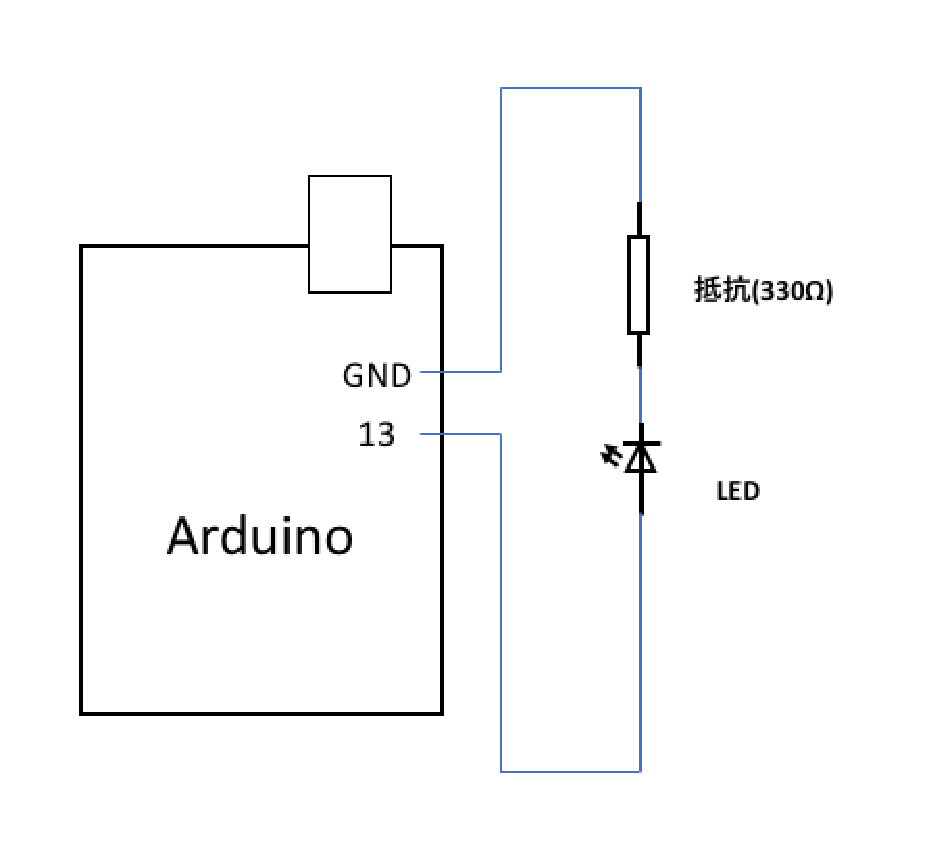
\includegraphics[width=60mm]{img/kairo2.eps}
  \caption{回路図}
 \end{minipage}
\end{figure}



\subsubsection*{プログラム}
\begin{lstlisting}
import processing.serial.*;
import cc.arduino.*;
 
Arduino arduino;
int ledPin = 13; // LED を接続したピンの番号
 
void setup() {
  arduino = new Arduino(this, Arduino.list()[5], 57600);

  // Arduino のピンモードを設定
  // ここでは 13 番ピンを Output 用に設定
  arduino.pinMode(ledPin, Arduino.OUTPUT);
}
 
void draw() {
  // Arduino の 13 番ピンを HIGH (5V) に
  arduino.digitalWrite(ledPin, Arduino.HIGH);
  delay(500); // 500ミリ秒間待つ

  // Arduino の 13 番ピンを LOW (0V) に
  arduino.digitalWrite(ledPin, Arduino.LOW);
  delay(500);
}
\end{lstlisting}

\newpage

\subsection{Processingの入力に応じてLEDを点灯させる}
Processingの画面上でマウスを押すとLEDが点灯するプログラムを作成してみましょう。Arduino側は、Digital Outの13番にLEDを接続しておきます。

\subsection*{mousePressed}
mousePressed 変数はマウスが押されているか押されていないかによって、それぞれ true と false に値が変わります。
これを用いると、「マウスがクリックされたときに何かをする」という動作が実現できます。

\begin{lstlisting}
 if (mousePressed) {
   // マウスが押されているときの処理
 } else {
   // マウスが押されていないときの処理
 }
\end{lstlisting}

\subsubsection*{プログラム}
\begin{lstlisting}
import processing.serial.*;
import cc.arduino.*;
 
Arduino arduino;
int ledPin = 13;
color bgColor = color(0);
 
void setup() {
  size(400, 200);
  arduino = new Arduino(this, Arduino.list()[5], 57600);
  arduino.pinMode(ledPin, Arduino.OUTPUT);
}
 
void draw() {
  if (mousePressed) {
    arduino.digitalWrite(ledPin, Arduino.HIGH);
    bgColor = color(255,0,0);
  }else{
    arduino.digitalWrite(ledPin, Arduino.LOW);
    bgColor = color(0);
  }
  background(bgColor);
}
\end{lstlisting}
画面をクリックすると、LEDが点灯します。

%\subsection*{スイッチを押すと LED が点灯するようにする}
%スイッチの入力を Processing で取得し、それに基づいて LED を制御しましょう。
%上 2 つの合わせ技です。

%これで入力と出力の両方が実現できるようになります。
%次回以降の実習でも入力や出力のための部品が変わるだけで基本的な考え方は同じです。


%\subsubsection*{TRY}
%今回やったことを思い出しながら、回路とプログラムを作成してみましょう。

% \subsubsection*{プログラムを書く}
% \begin{lstlisting}
% import processing.serial.*;
% import cc.arduino.*;

% Arduino arduino;
% int ledPin = 13;
% int switchPin = 8;
 
% void setup() {
%   size(400, 300);
%   arduino = new Arduino(this, Arduino.list()[0], 57600);
%   arduino.pinMode(switchPin, Arduino.INPUT);
%   arduino.pinMode(ledPin, Arduino.OUTPUT);
% }
 
% void draw() {
%   if (arduino.digitalRead(switchPin) == Arduino.HIGH) {
%     background(255, 0, 0);
%     arduino.digitalWrite(ledPin, Arduino.HIGH);
%   } else {
%     background(0, 0, 0);
%     arduino.digitalWrite(ledPin, Arduino.LOW);
%   }
% }
% \end{lstlisting}


%\subsection*{mousePressed}
%mousePressed 変数はマウスが押されているか押されていないかによって、それぞれ true と false に値が変わります。
%これを用いると、「マウスが押されているときに何かをする」という動作が実現できます。
%
%\begin{lstlisting}
% if (mousePressed) {
%   // マウスが押されているときの処理
% } else {
%   // マウスが押されていないときの処理
% }
%\end{lstlisting}
%
%では、下のプログラムを参考にしてマウスが押されている間 LED が点灯する、というプログラムを書いてみましょう。
%
%回路は前回のままで OK です。
%
%\begin{lstlisting}
%import processing.serial.*;
%import cc.arduino.*;
% 
%Arduino arduino;
%int ledPin = 13;
% 
%void setup() {
%  arduino = new Arduino(this, Arduino.list()[5], 57600);
%  arduino.pinMode(ledPin, Arduino.OUTPUT);
%}
% 
%void draw() {
%  if (mousePressed) {
%    // ここに命令を追加する
%  } else {
%    // ここに命令を追加する
%  }
%}
%\end{lstlisting}
%
%\subsubsection*{ヒント}
%\begin{lstlisting}
% arduino.digitalWrite(n, Arduino.HIGH); // n 番ピンを High (5V) に
% arduino.digitalWrite(n, Arduino.LOW);  // n 番ピンを Low (5V) に
%\end{lstlisting}
%

\newpage
\section{Digital Input}
ここからが本題です。
Arduino の Digital Input を用いてスイッチの ON/OFF を取得してみましょう。

\subsection*{プルアップ/プルダウン抵抗}
デジタル回路の場合、入力端子がどこにも接続されていないような状態 (オープン) が起こると、電圧が High (5V) または Low (0V) に定まらず誤動作の原因になります。
そのため、マイコンの入力信号がHighかLowかを確実に伝えるために、プルアップ/プルダウン抵抗が必要となります。

%例えスイッチはOFFの状態でも、静電気や電磁誘導によって、電流が生じてしまう。
%マイコンの入力信号がHigh(5V)かLow(0V)かを確実に伝えるために、プルアップ/プルダウン抵抗が必要となります。

\subsection{プルアップ抵抗}
図\ref{fig:pullup}を見ると、5V側に抵抗が付いています。これをプルアップ抵抗と言います。
 
スイッチが押されていない時、Arduinoは図\ref{fig:pullup} (左) のように抵抗を通して5VとつながるのでHIGH (5V) になります。

スイッチが押されている時、Arduinoは図\ref{fig:pullup} (右) のようにスイッチを通してGNDとつながるのでLOW (0V) になります。電流は青い線のように流れ、Arduinoには流れません。

\begin{figure}[htbp]
 \begin{minipage}{0.5\columnwidth}
  \centering
  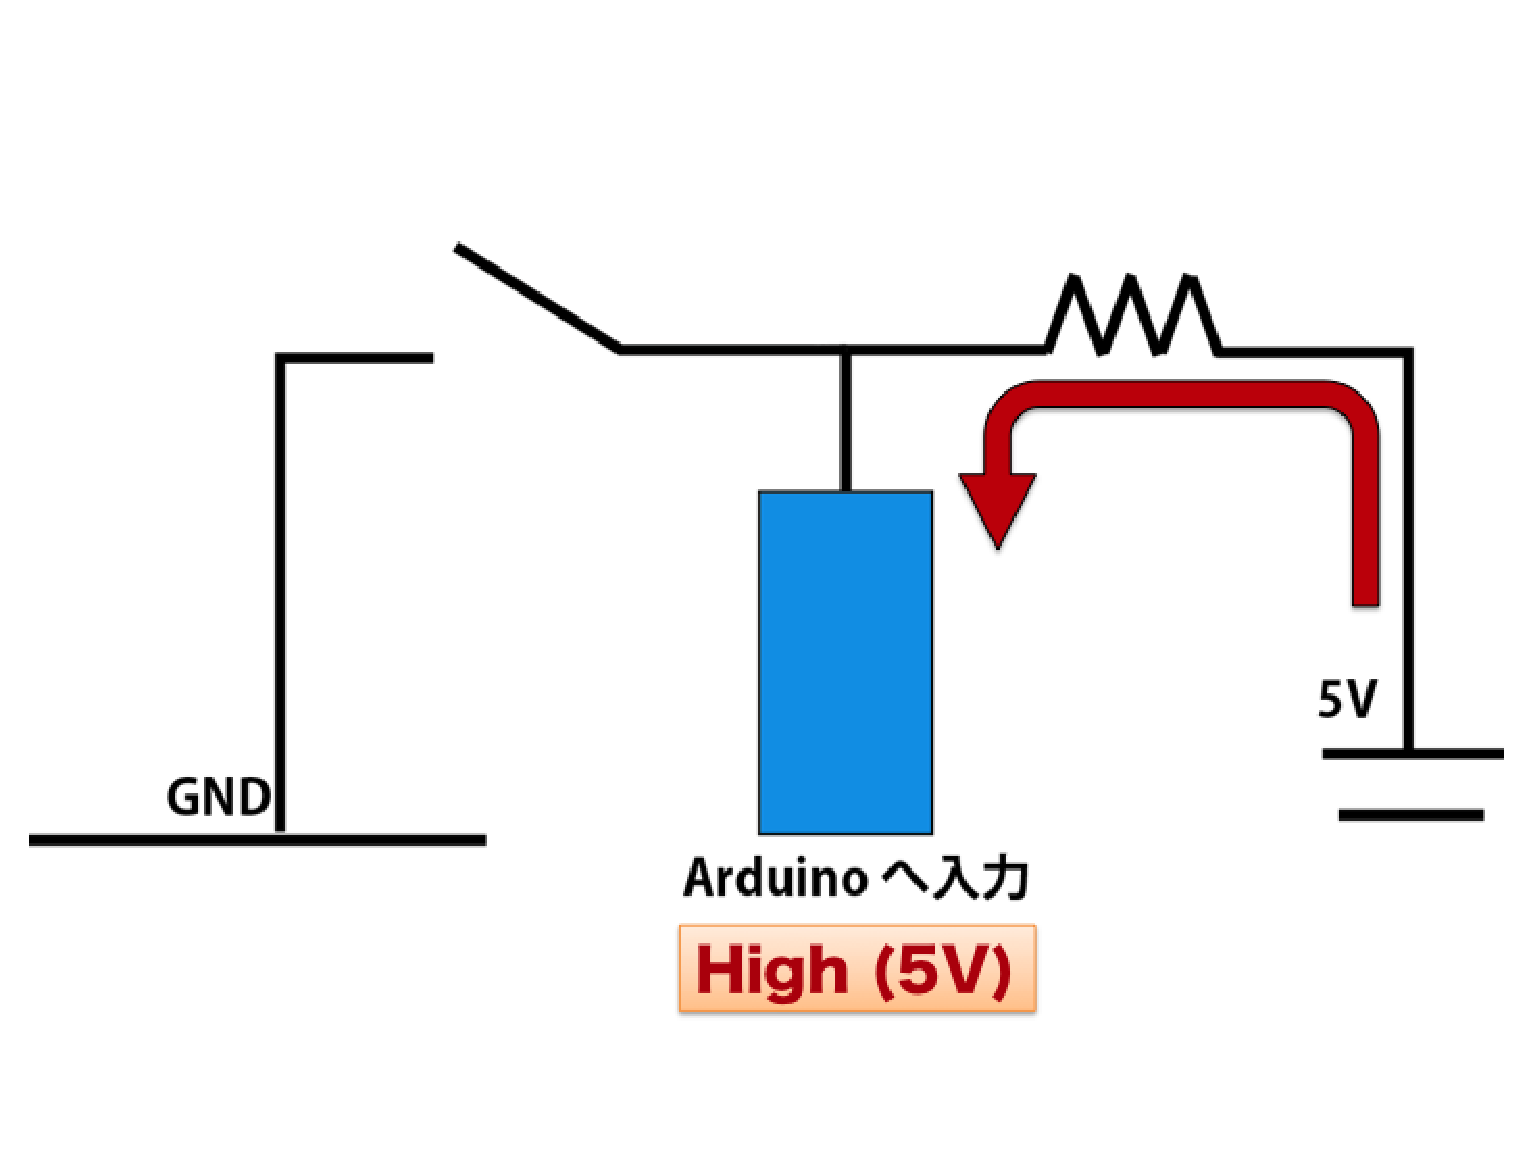
\includegraphics[width=0.8\columnwidth]{img/pullup_off.eps}
 \end{minipage}
 \begin{minipage}{0.5\columnwidth}
  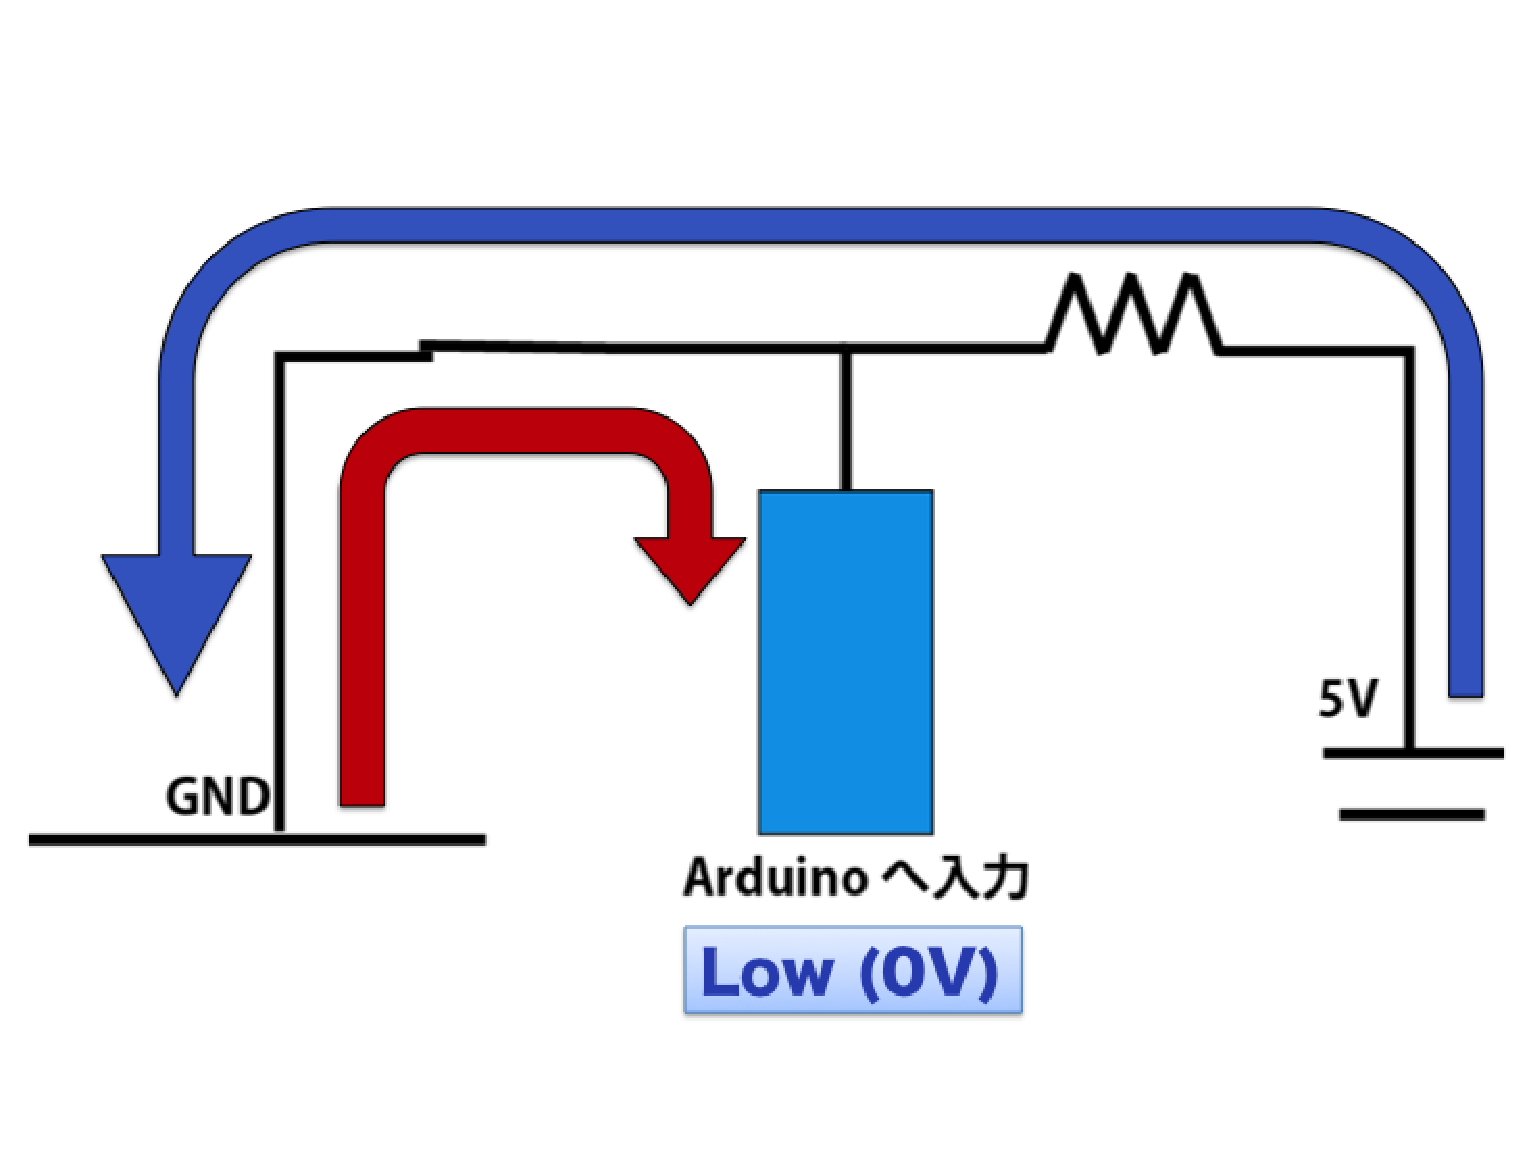
\includegraphics[width=0.8\columnwidth]{img/pullup_on.eps}
 \end{minipage}
 \caption{プルアップ回路 スイッチOFF時 (左) とON時 (右)  }
 \label{fig:pullup}
\end{figure}

%\begin{figure}[h!]
% \begin{minipage}{0.5\columnwidth}
%  \centering
% 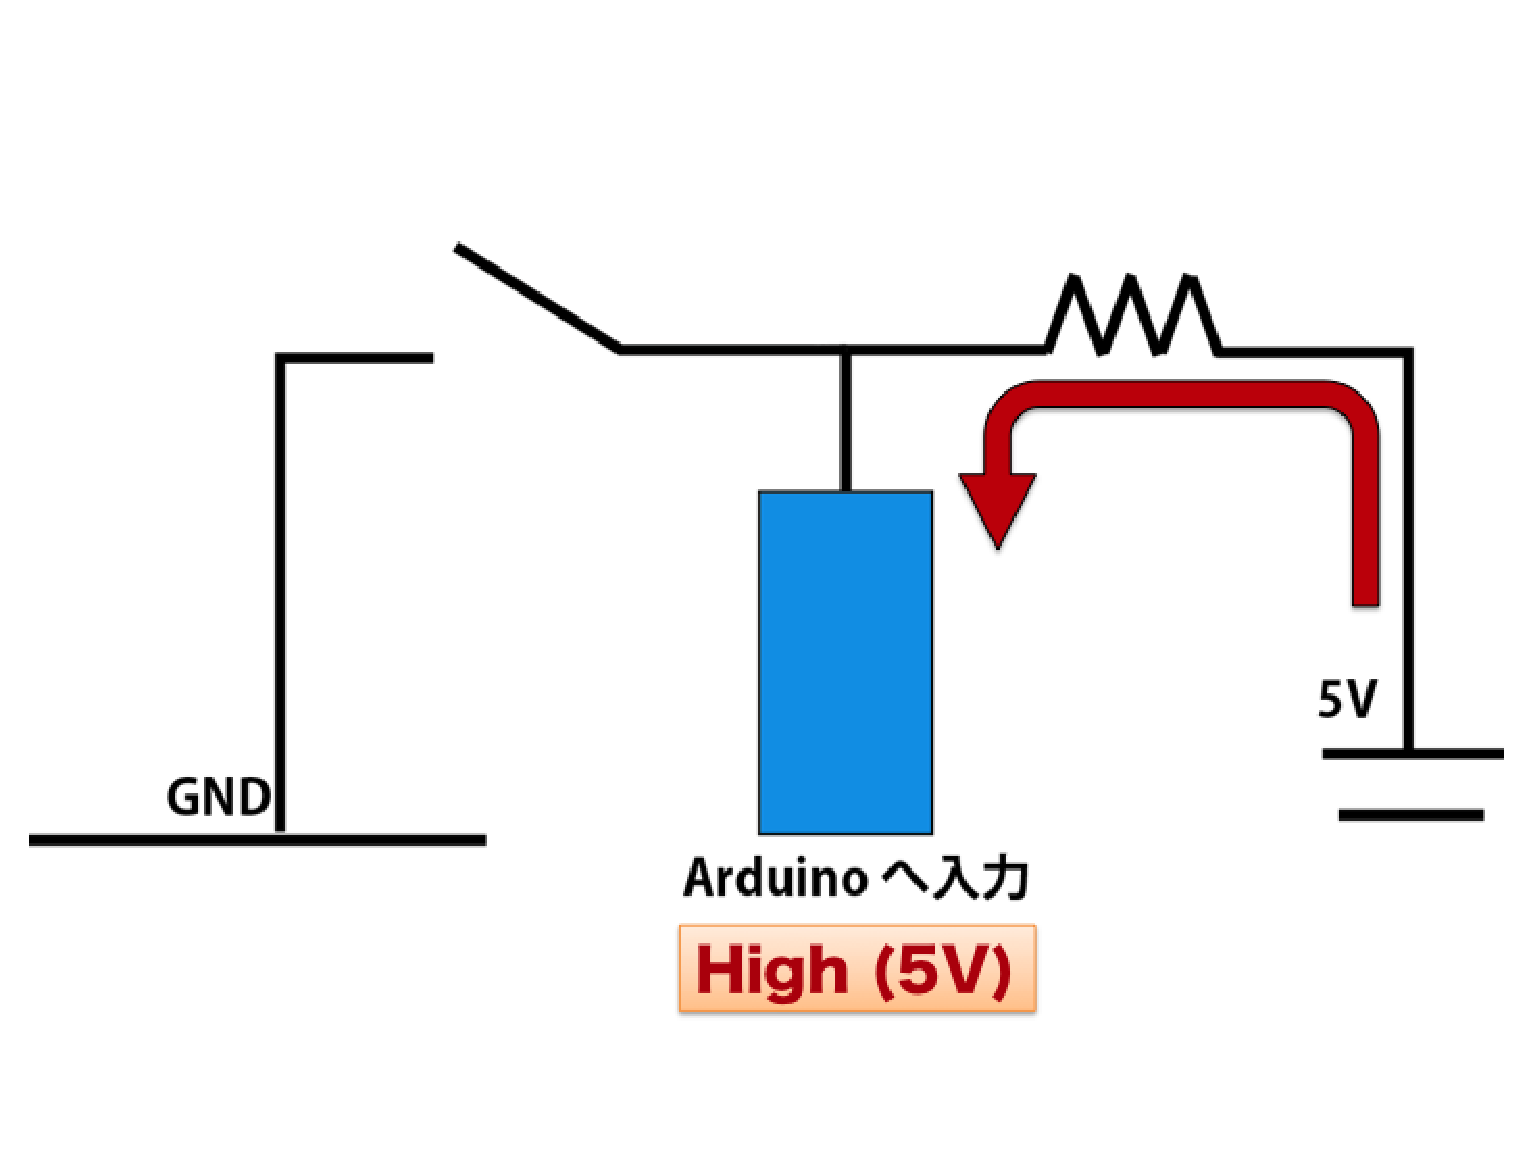
\includegraphics[width=0.9\columnwidth]{img/pullup_off.eps}
% \end{minipage}
% \begin{minipage}{0.5\columnwidth}
%  \centering
%  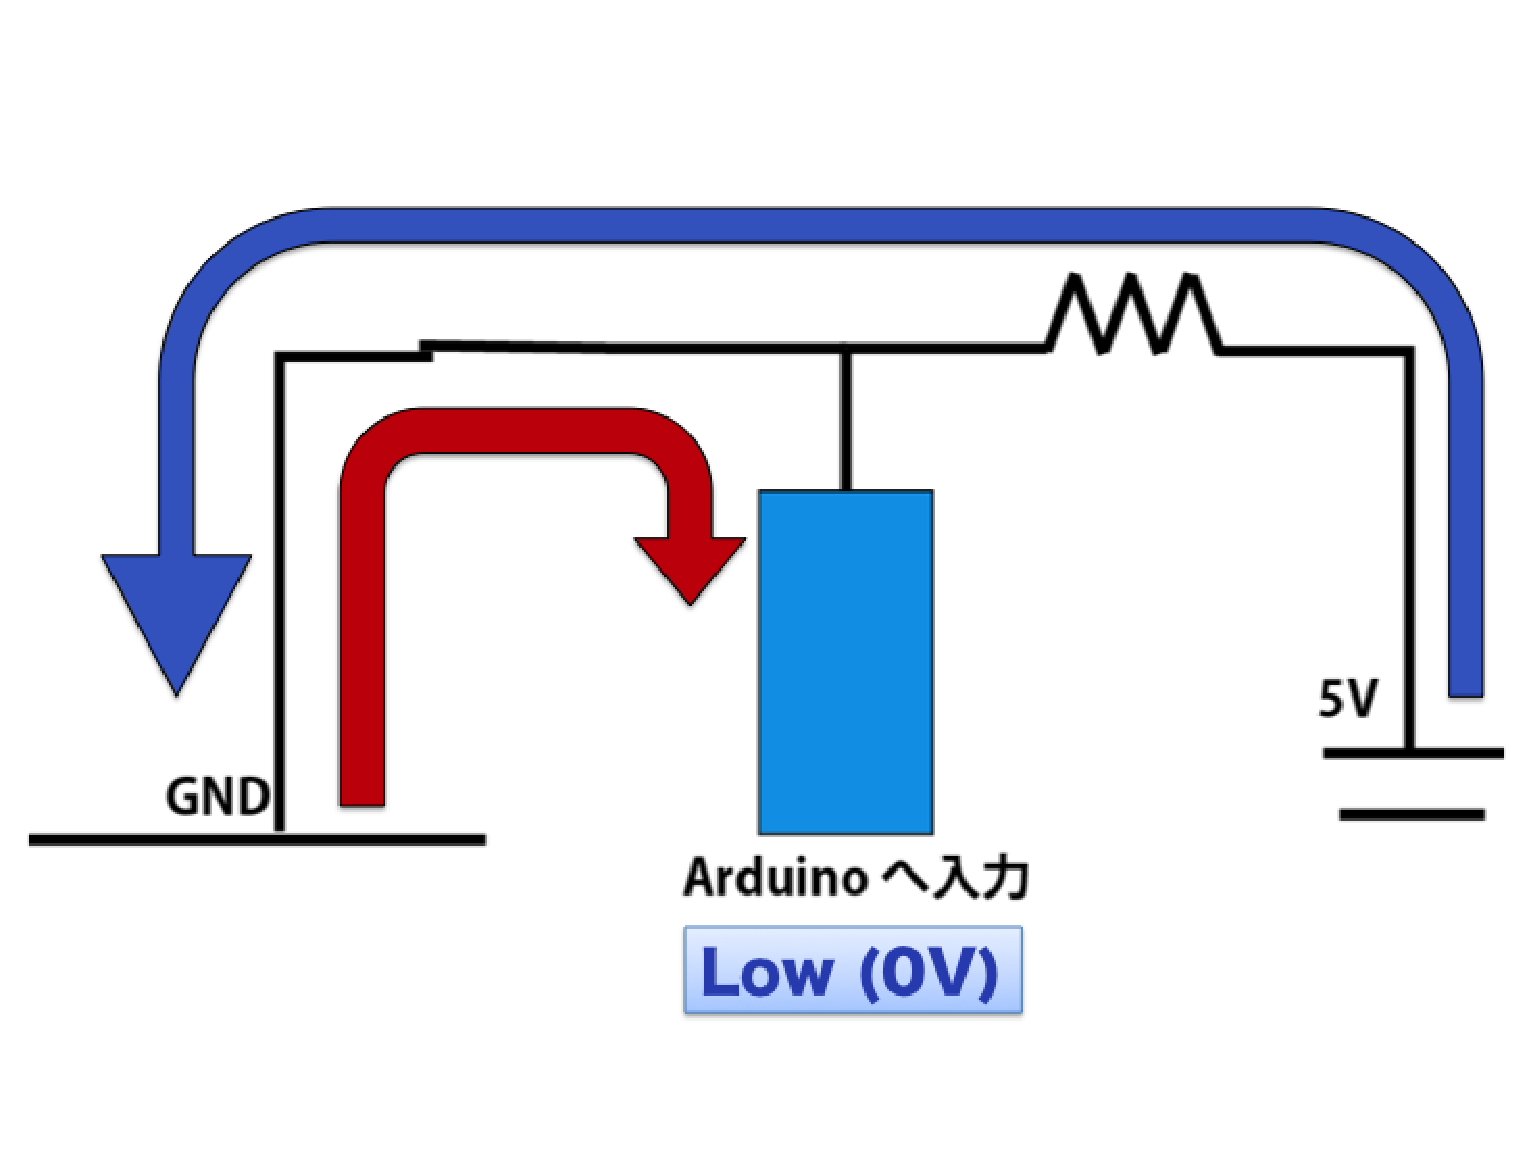
\includegraphics[width=0.9\columnwidth]{img/pullup_on.eps}
%\end{minipage}
%  \caption{プルアップ抵抗ON (左) OFF (右)}
%\end{figure}


\subsection{プルダウン抵抗}
 図\ref{fig:pulldown}を見ると、GND側に抵抗が付いています。これをプルダウン抵抗と言います。
 
 スイッチが押されていない時、Arduinoは図\ref{fig:pulldown} (左) のように抵抗を通してGNDとつながるので、LOW (0V) になります。
 
 スイッチが押されている時、Arduinoは図\ref{fig:pulldown} (右) のようにスイッチを通して5Vとつながるので、HIGH (5V) になります。

 \begin{figure}[htbp]
  \begin{minipage}{0.5\columnwidth}
   \centering
   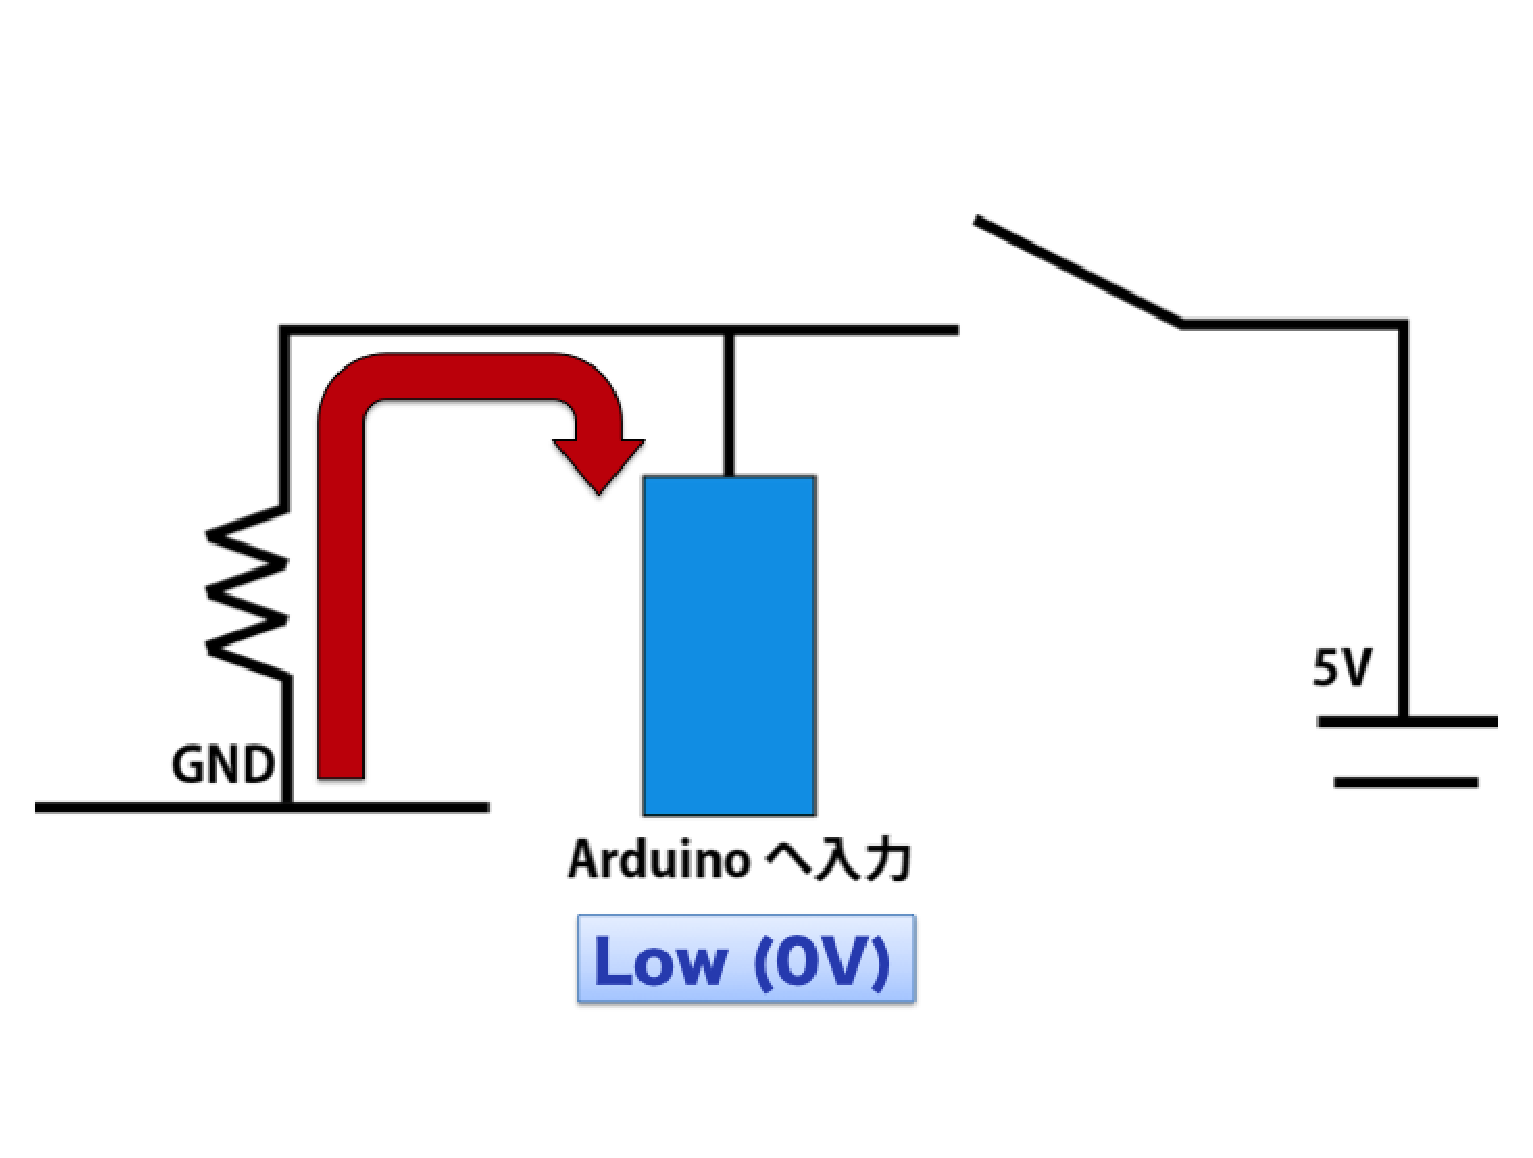
\includegraphics[width=0.8\columnwidth]{img/pulldown_off.eps}
  \end{minipage}
  \begin{minipage}{0.5\columnwidth}
   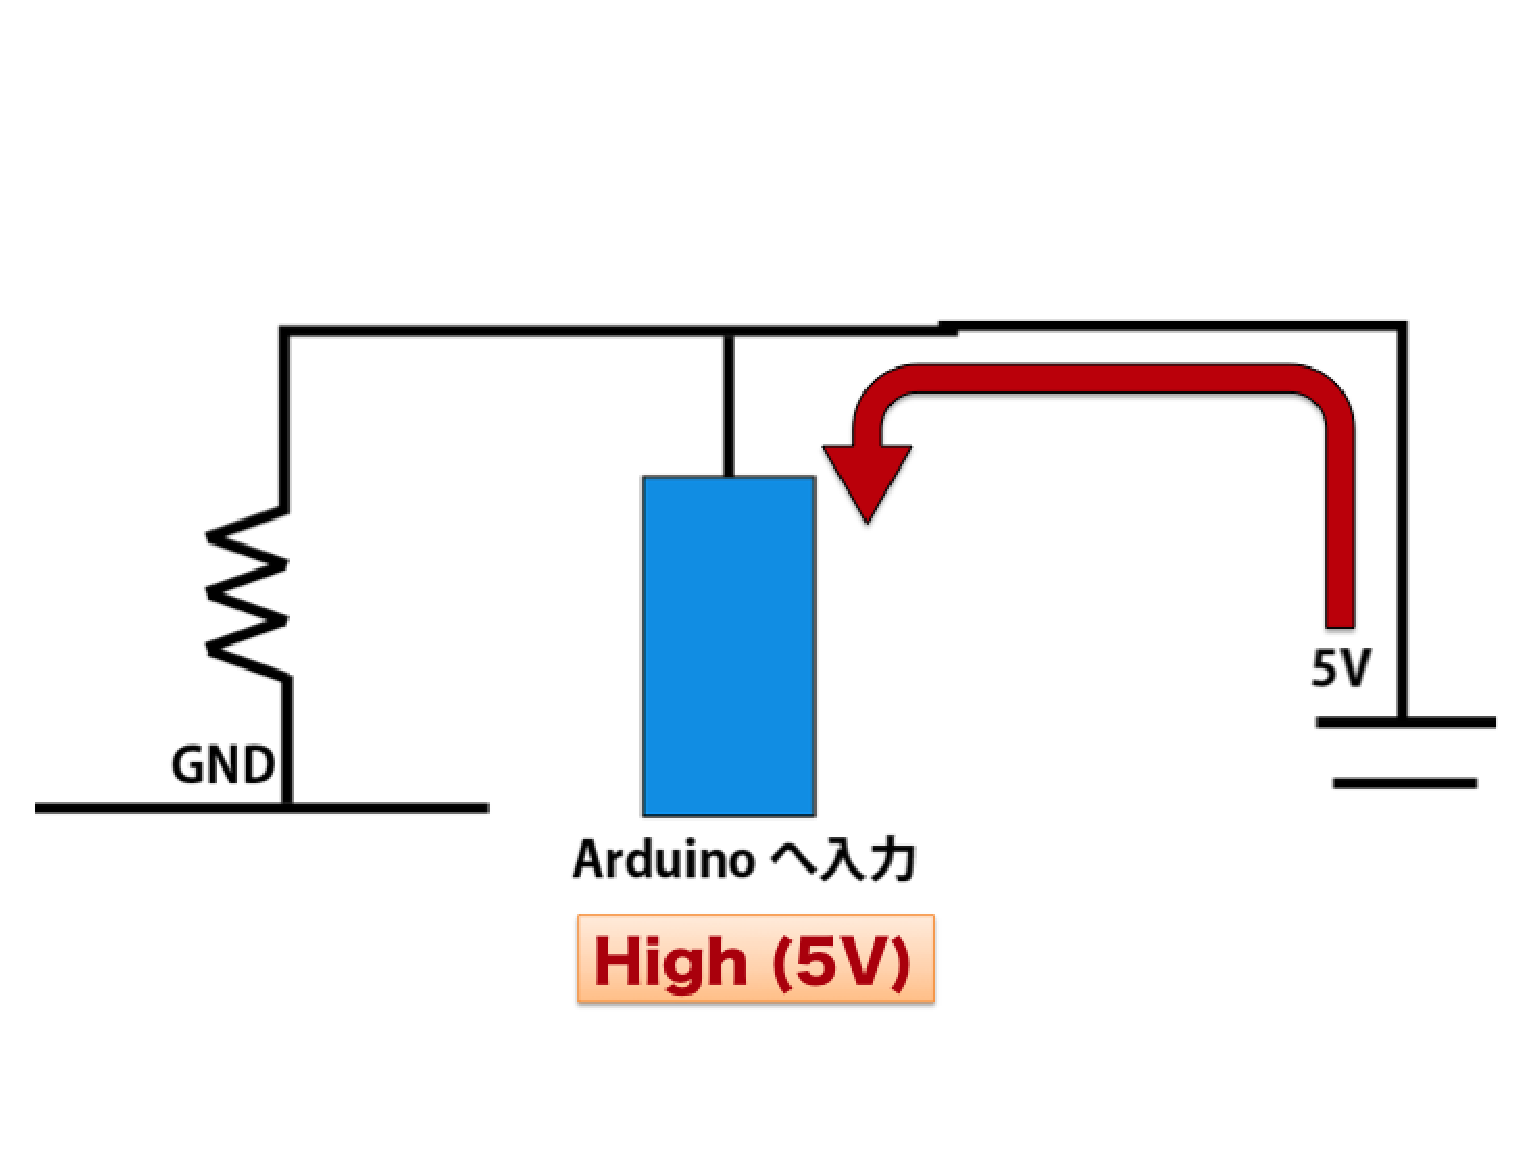
\includegraphics[width=0.8\columnwidth]{img/pulldown_on.eps}
  \end{minipage}
  \caption{プルダウン回路 スイッチOFF時 (左) とON時 (右)  }
  \label{fig:pulldown}
\end{figure}

%\begin{figure}[h!]
% \begin{minipage}{0.5\columnwidth}
  %\centering
 % 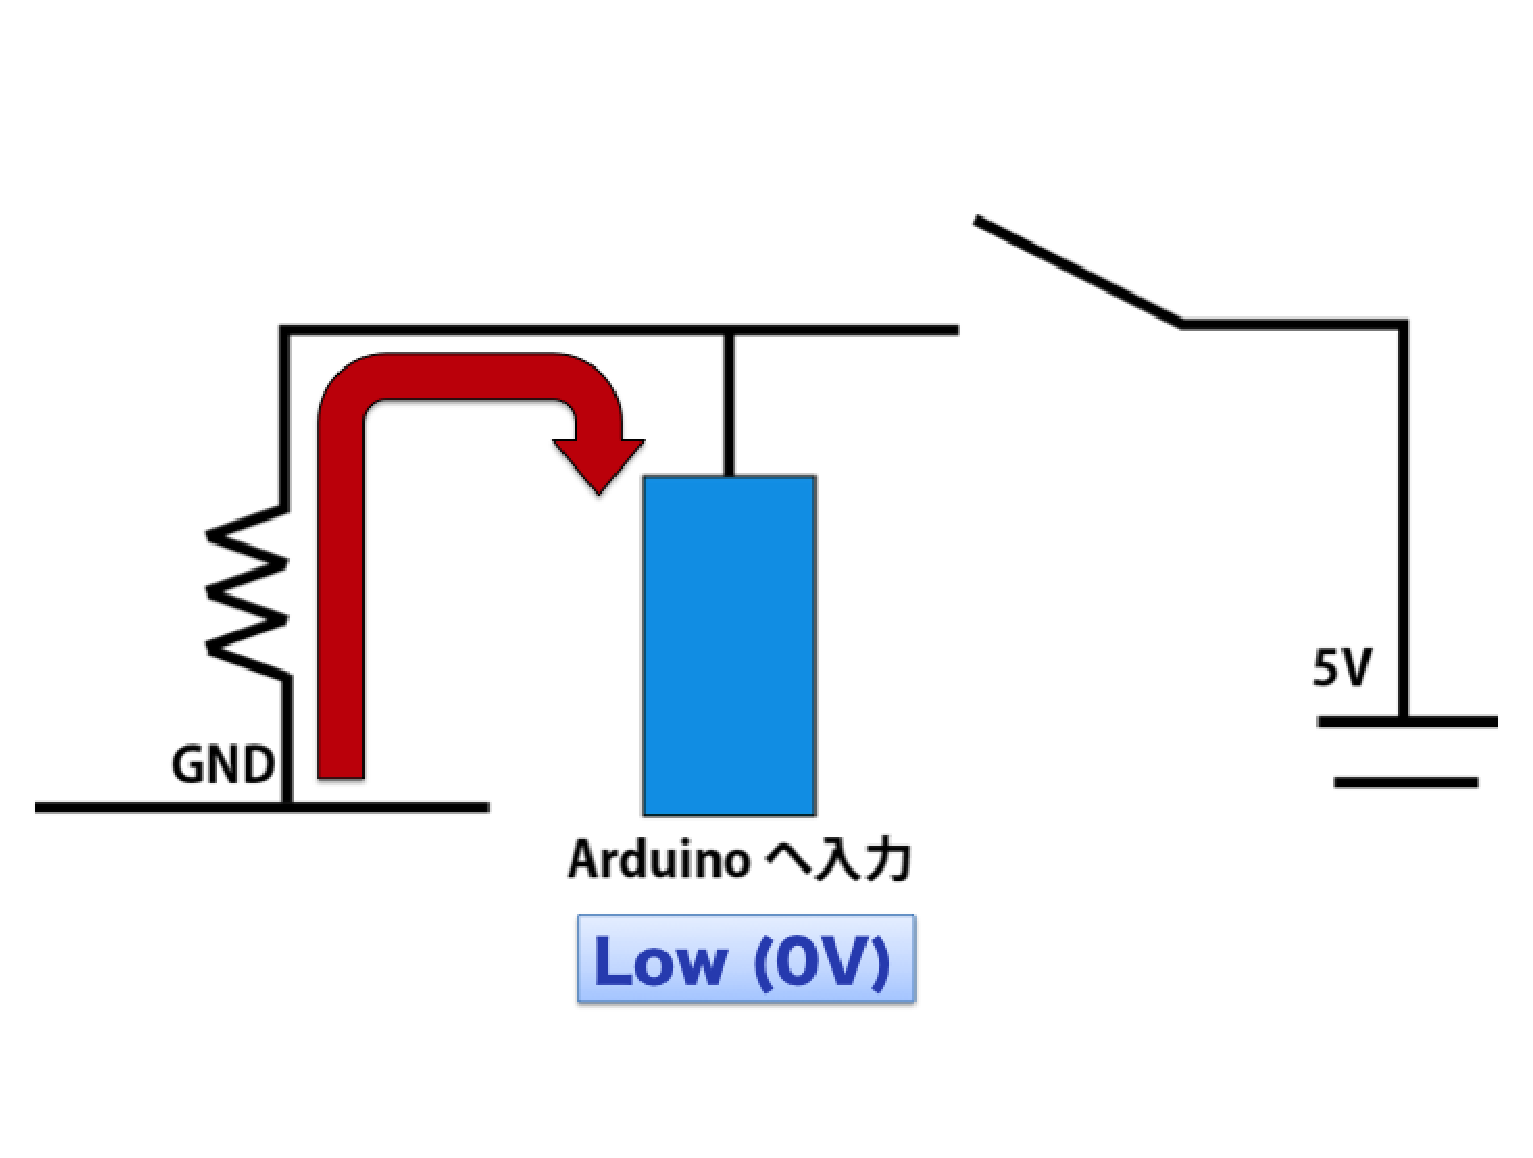
\includegraphics[width=0.9\columnwidth]{img/pulldown_off.eps}
% \end{minipage}
% \begin{minipage}{0.5\columnwidth}
 % \centering
 % 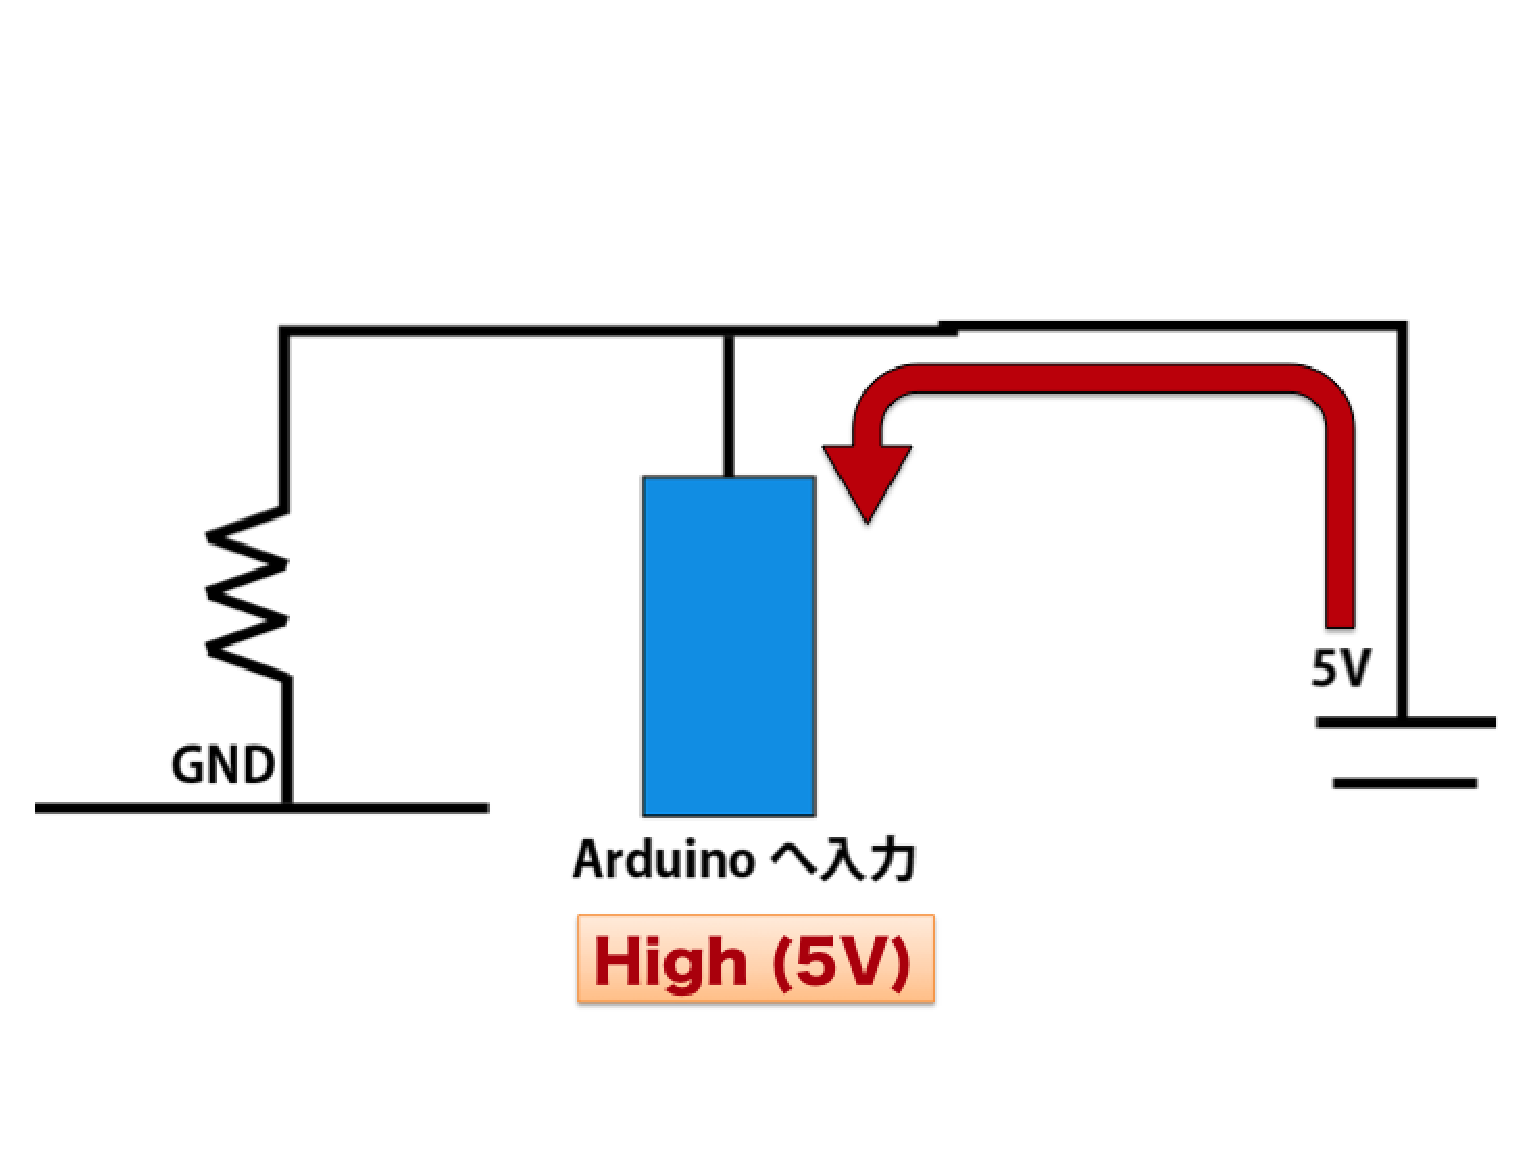
\includegraphics[width=0.9\columnwidth]{img/pulldown_on.eps}
 %\end{minipage}
 % \caption{プルダウン抵抗ON (左) OFF (右)}
%\end{figure}

\newpage

\subsection{回路}
\begin{figure}[htbp]
 \begin{minipage}{0.5\columnwidth}
  \centering
  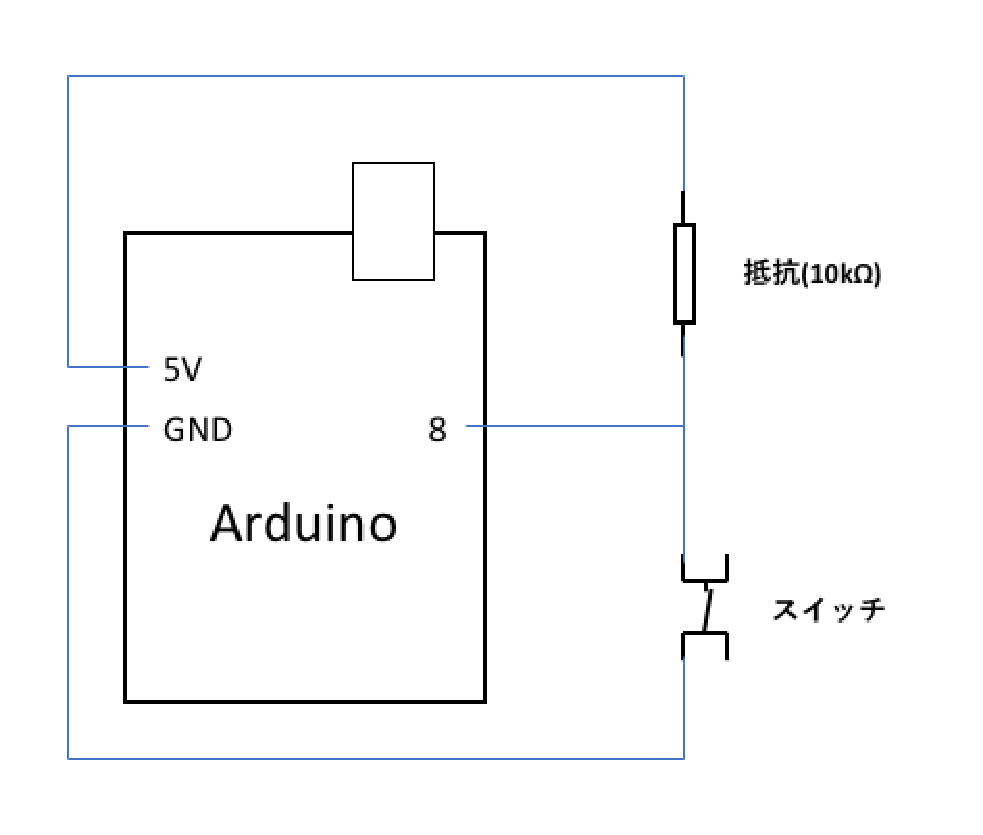
\includegraphics[width=0.62\columnwidth]{img/pull_up.eps}
 \end{minipage}
 \begin{minipage}{0.5\columnwidth}
  \centering
  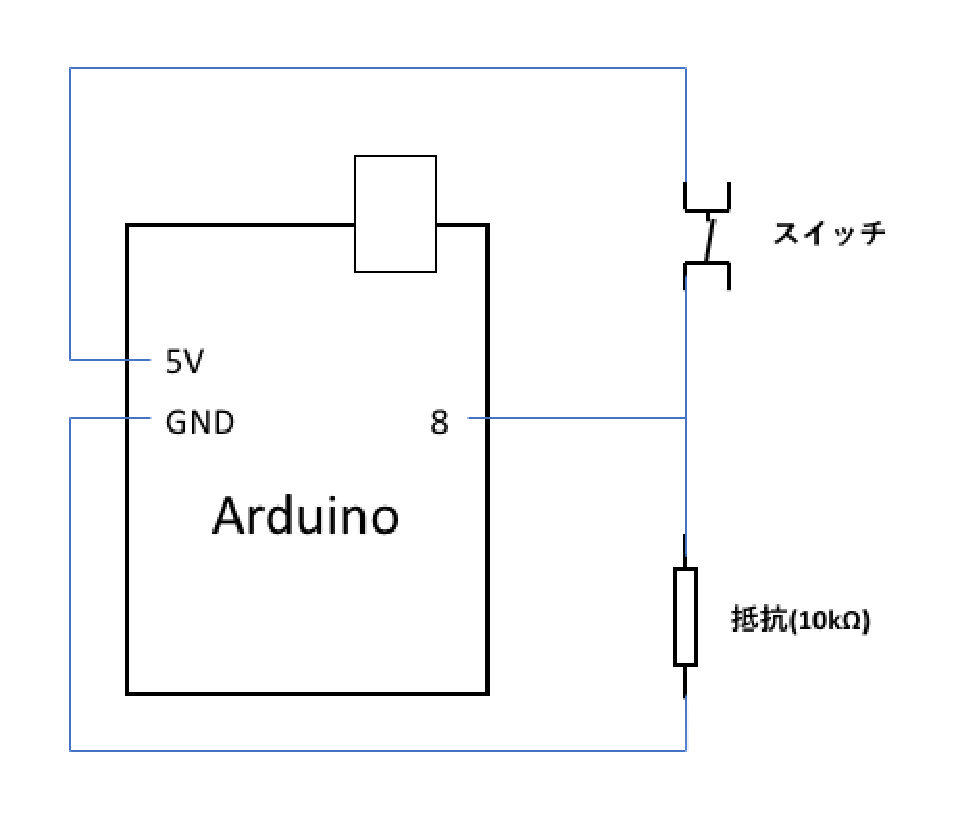
\includegraphics[width=0.62\columnwidth]{img/pull_down.eps}
 \end{minipage}
  \caption{プルアップ抵抗 (左) とプルダウン抵抗 (右)}
\end{figure}


\subsection{プログラム}
\begin{lstlisting}
import processing.serial.*;
import cc.arduino.*;

Arduino arduino;
int switchPin = 8; // スイッチを接続したピンの番号
 
void setup() {
  size(400, 300);
  arduino = new Arduino(this, Arduino.list()[5], 57600);
  arduino.pinMode(switchPin, Arduino.INPUT); // ピンモードを Input に
}
 
void draw() {
  // 8番ピンの電圧を取得し、それが HIGH ならば
  if (arduino.digitalRead(switchPin) == Arduino.HIGH) {
    background(255, 0, 0); // 背景を赤に
  } else {
    background(0, 0, 0);   // そうでなければ (LOW ならば) 背景を黒に
  }
}
\end{lstlisting}

\section{Digital Input と Digital Output を組み合わせる}
スイッチの入力を Processing で取得し、それに基づいて LED を制御しましょう。
前回やった Digital Input と今回やった Digital Output の合わせ技です。

これで入力と出力の両方が実現できるようになります。
次回以降の実習でも入力や出力のための部品が変わるだけで基本的な考え方は同じです。

\subsection{スイッチの ON/OFF に応じてLEDを点灯させる}
Digital Inputと Digital Output を用いてスイッチの ON/OFF に応じてLEDを点灯させてみましょう。

\subsection{スイッチを押している間だけLEDを点滅させる (上級編) }
Digital Inputと Digital Output を用いてスイッチを押している間だけ LEDを1秒間隔で点滅させてみましょう。

\subsection*{TRY}
%前回と今回やったことを思い出しながら、回路とプログラムを作成してみましょう。
今回やったことを思い出しながら、回路とプログラムを作成してみましょう。
\end{document}

